\chapter{Architectural Design}
\label{cha:arch}
\section{Overview}
\label{sec:overview}
This section presents a panoramic overview of the architectural component of the application.
Beginning with a high-level approach towards a more detailed and deeper level of the technologies.
We will discuss the how and why we have chosen the technologies that we will use in the development of the clients and which backend solution.
\newline Travlendar+ will rely on the AWS technology, that will allow us a fast development phase and a modular scalability. 
This will enable to have a degree of flexibility that cannot be achieved through hosting and implementing our own architecture in the traditional way.
Accessing the AWS services is going to be doable thanks to the AWS SDK's available that helps to take out of coding the complexity of accessing them providing wrapped APIs in every major technology that could be used to implement the clients.
In our case, the mobile clients will be implemented with the Xamarin.Forms technology that will help us to achieve a multi-platform solution with an excellent code-sharing approach.
Xamarin.Forms allow us to develop quickly native iOS/Android/Windows applications in C\# having native UI elements and access to platform-specific APIs.
The web application will be based on Angular.js and HTML5.
Angular.js is one of the most popular JavaScript frameworks for web applications, it allows to have a rapid development and its maintained by Google Engineers meaning that you will find reliable support if needed.
It perfectly integrates with HTML5 and its fully compatibly with the MVVM approach

\begin{figure}[H]
	\centering
	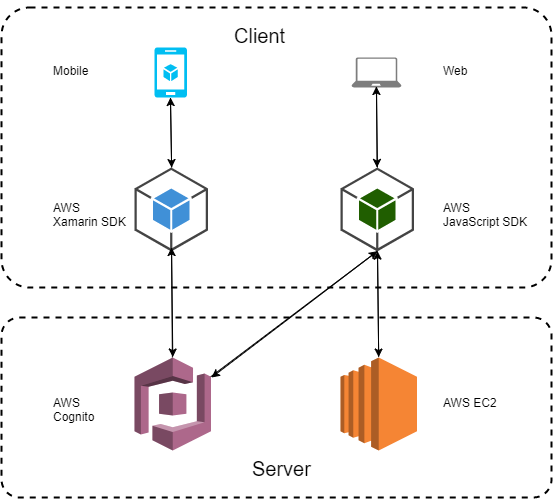
\includegraphics[width=4in]{diagrams/ArchitectureDiagram.png} 
	\caption{Architecture Diagram.}   
\end{figure}

\section{Component view}
\label{sec:comp_view}
The following views will cover the major components and technologies that the system uses.

\textbf{Client:} Implementation of the application that makes requests to the server and will be provided with a response. In Travlendar+ the clients will be the mobile application and the web application, that interacts with the server through REST APIs.

\textbf{Server:} Layer that provides the workflow and the business logic for the client applications. It will be implemented with AWS technologies interacting with a different component for each type of client.

\textbf{Web Server:} Software running on a server able to communicate with web application clients using the HTTP (or HTTPS) protocol.

\textbf{Application Server:} Server that provides the infrastructure and the functionalities needed to the application

\textbf{AWS:} Cloud services that offer computing power, database storage, content delivery and other scalable functionalities.

\textbf{Xamarin:} Technology that delivers native Android, iOS and Windows applications using a shared C\# codebase and the same APIs.

\textbf{Web Browser:} Application for retrieving and presenting web pages and applications.

\subsection*{Server-side application}

Travlendar+ will rely on AWS services.
Our main core service is Amazon Cognito Sync that will allow us to sync the user's data across multiple clients and platforms.
The login will be managed by the Amazon Cognito Identity service and it will implement either the social platforms authentications (Facebook and Google) and through the traditional email registration flow.
This is feasible associating an identity with a dataset containing key-values pairs having a maximum size of 1 MB. Due to AWS limitations, each identity can be associated with maximum 20 datasets.
Amazon Cognito Sync will create a local cache for the identity data. 
The application will interact with this local cache when is reading or writing the keys. 
This allows Travlendar+ to synchronize all the changes made on a device immediately to other devices.
We will store not only the user preferences but also the user events and means of transports, this could be enhanced in future to other services using Amazon Cognito towards an AWS DynamoDB or and AWS Lambda if we would like to transfer some computational power towards the backend side.
Amazon Cognito offers a scalable and modular way to react upon peaks in demands and traffic.

\subsection*{Mobile client application}
The Travlendar+ mobile implementation will be done with Xamarin technologies. 
This will allow us having a multiplatform presence and speeding up the development phase while maintaining a good degree of modularity.
Due to this choice, we will have to use the .NET version of the SDKs that we need and whenever it's not possible we have to bind the native Android and iOS libraries.
We will use the Xamarin.Forms framework, that is a cross-platform UI toolkit that allows us to create a native interface. 
We can choose to use the main control groups to create the User Interface, which are Pages, Layouts, Views and Cells that will be mapped and rendered to the native equivalent.
Whenever needed a customized UI component we can use a platform-specific view built with Xamarin.iOS or Xamarin.Android.
Xamarin.Forms applications are architected in the same way as any other cross-platform application. 
There are two viable approaches, the most common is with Portable Class Libraries (PCL) while the other is via Shared Projects.
Our choice is towards the PCL that will result in a DLL usable on the specific platforms for which we provide support.
This approach has a number of advantages like a centralized code base consumed by the platform projects, refactor operation will affect all the code within the solution and the relief of referencing itself against the platform projects. 
The downside will concern platform specific libraries, which cannot be referenced inside the PCL. This can be avoided using the Dependency Injection pattern, using an interface in the Portable Class passing platform-specific features.
\begin{figure}[H]
	\centering
	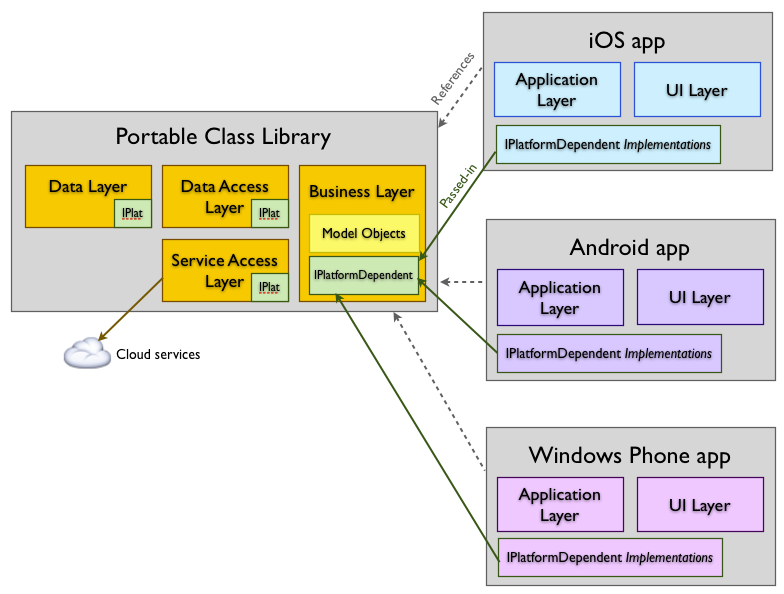
\includegraphics[width=6in]{diagrams/PCLDiagram.png} 
	\caption{PCL Diagram.}   
\end{figure}

\subsection*{Web application}

\subsection*{Database}

\section{Deployment view}
\label{sec:depl_view}

\section{Runtime view}
\label{sec:runtime_view}

\begin{figure}
	\centering
	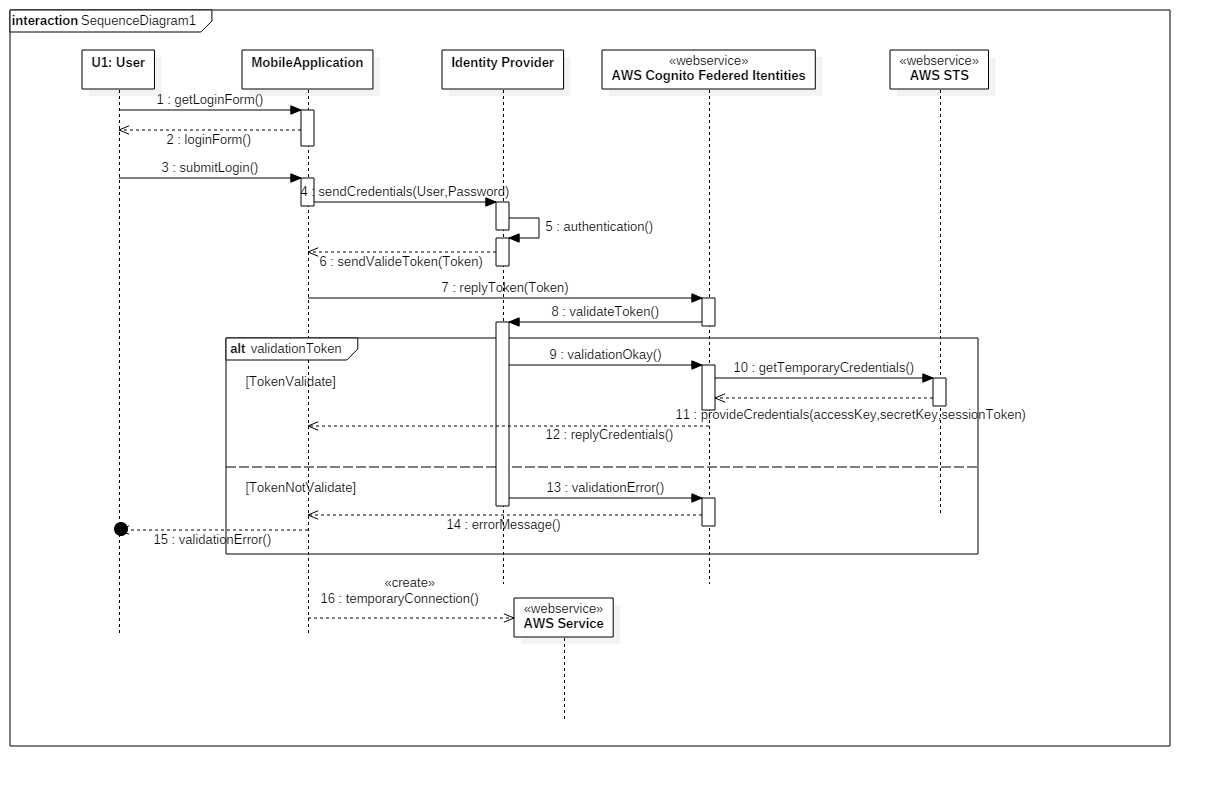
\includegraphics[width=6in]{./diagrams/SequenceDiagramLogin.png}
	\caption{Sequence diagram of the login with the AWS Web Service}
	\label{fig:seqLogin}
\end{figure}

\section{Component interfaces}
\label{sec:runtime_view}

\section{Selected architectural styles and patterns}
\label{sec:archs}

\section{Other design decisions}
\label{sec:des_dec}